\documentclass[aspectratio=169]{beamer}

\usepackage[utf8]{inputenc}
\usepackage[croatian]{babel}
\usepackage{booktabs}
\usepackage{pgfplots}
\usepackage{hyperref}
\usepackage{tikz}
\usepackage{graphicx}
\usetikzlibrary{positioning}
\pgfplotsset{compat=1.18}

\usetheme{Madrid}
\usecolortheme{default}
\setbeamertemplate{navigation symbols}{}
\setbeamertemplate{caption}[numbered]

\title[Bots and how to catch them]{Bots and how to catch them}
\subtitle{Detekcija AI-generiranih Reddit komentara}
\author{STEM Games 2026 -- Mathematics arena x Erste}
\date{2026}

\begin{document}

\begin{frame}
    \titlepage
\end{frame}

\begin{frame}{Uvod}
    \begin{itemize}
    \item Društvene mreže -- danas više od 5,4 milijarde korisnika
    \item Značaj dio prometa čine botovi (good i bad)
    \item Problem bad botova -- ozbiljna društvena prijetnja
    \item Spam, phishing, manipulacija raspravama i umjetno povećanje
angažmana
    \item Dead internet theory

    \end{itemize}
\end{frame}

\begin{frame}{Ukupan udio botova na webu}
    \centering
    \begin{center}
    \begin{tikzpicture}
        \begin{axis}[
            title={Ukupan udio botova (Bad + Good Bots)},
            xlabel={Godina},
            ylabel={Udio prometa (\%)},
            xmin=2012, xmax=2028,
            ymin=30, ymax=65,
            xticklabel style={/pgf/number format/set thousands separator={}},
            xtick={2013, 2015, 2017, 2019, 2021, 2023, 2025, 2027},
            grid=both,
            minor tick num=1,
            legend pos=north west,
            width=0.88\textwidth,
            height=0.62\textheight,
        ]
            \addplot[teal, only marks, mark=square*, mark size=2pt] coordinates {
                (2013, 43.0) (2014, 57.1) (2015, 45.6) (2016, 38.7)
                (2017, 42.2) (2018, 37.9) (2019, 37.2) (2020, 40.8)
                (2021, 42.3) (2022, 47.4) (2023, 49.6) (2024, 51.0)
                (2025, 53.0)
            };
            \addlegendentry{Ukupni podaci}

            \addplot[orange, ultra thick, domain=2013:2028, samples=100] {0.15814*x^2 - 639.186*x + 645164};
            \draw[magenta, dashed, line width=1pt] (axis cs:2012,50) -- (axis cs:2028,50) node[pos=0.1, above, scale=0.7]{50\%};
        \end{axis}
    \end{tikzpicture}
    
    \vspace{1mm}
        {\tiny Izvor: Statista, Human and bot web traffic share}
    \end{center}
\end{frame}



\begin{frame}{Uspon ``bad bot'' prometa}
    \centering
    \begin{tikzpicture}
        \begin{axis}[
            title={Kvadratna aproksimacija rasta ``Bad Bot'' prometa},
            xlabel={Godina},
            ylabel={Udio prometa (\%)},
            xmin=2012, xmax=2028,
            ymin=15, ymax=55,
            xticklabel style={/pgf/number format/set thousands separator={}},
            xtick={2013, 2015, 2017, 2019, 2021, 2023, 2025, 2027},
            grid=both,
            minor tick num=1,
            legend pos=north west,
            width=0.88\textwidth,
            height=0.62\textheight,
        ]
            \addplot[blue, only marks, mark=*, mark size=2pt] coordinates {
                (2013, 23.6) (2014, 22.8) (2015, 18.6) (2016, 19.9)
                (2017, 21.8) (2018, 20.4) (2019, 24.1) (2020, 25.6)
                (2021, 27.7) (2022, 30.2) (2023, 32.0) (2024, 37.0)
                (2025, 40.0)
            };
            \addlegendentry{Bad Bot podaci}

            \addplot[red, ultra thick, domain=2013:2027.5, samples=100] {0.21*(x-2015.5)^2 + 19.5};
            \addlegendentry{Trend rasta}
            \draw[magenta, dashed, line width=1pt] (axis cs:2012,50) -- (axis cs:2028,50) node[pos=0.9, above, scale=0.7]{50\%};
            
        \end{axis}
    \end{tikzpicture}
    
    \vspace{1mm}
    {\tiny Izvor: Statista, Human and bot web traffic share}
\end{frame}



\begin{frame}{Ključne metrike bot prometa}
    \centering
    \small
    \begin{tabular}{@{}llc@{}}
        \toprule
        \textbf{Kategorija} & \textbf{Metrika} & \textbf{Vrijednost} \\ \midrule
        \textbf{Promet} & Udio botova u ukupnom prometu & 53\% \\
         & Udio ljudskog prometa & 47\% \\
        \textbf{Sigurnost} & Udio ``loših'' botova & 40\% \\
         & Godišnji porast AI bot napada & 12.5x \\
        \textbf{Infrastruktura} & Bot napadi na API-je & 27\% \\
         & Bot napadi na poslovnu logiku & 21\% \\
        \textbf{Metode} & Botovi koji koriste Chrome za prikrivanje & 41\% \\
        \textbf{Industrija} & Napadi na financijske usluge & 24\% \\
         & Preuzimanje računa u financijama & 46\% \\ \bottomrule
    \end{tabular}

    \vspace{2mm}
    {\tiny Izvor: Thales/Imperva, Bad Bot Report 2026}
\end{frame}


\begin{frame}{Projekt}
    \begin{itemize}
        \item  Detekcija i procjena vjerojatnosti AI generiranih komentara i objava
        \item Stvaramo sustav koji spaja tri komplementarna pogleda u ansambl modela (ensemble learning)
        \item Semantički pogled na značenje komentara, strukturni pogled na gradu rečenica i interpunkciju te
leksički pogled na riječi, tokene i kratke znakovne obrasce
        \item Završni stacking meta-model (kombinira 3 podsustava)
    \end{itemize}
\end{frame}

\section{Detekcijski Sustav}

\begin{frame}{Naš detekcijski sustav}
    \centering
    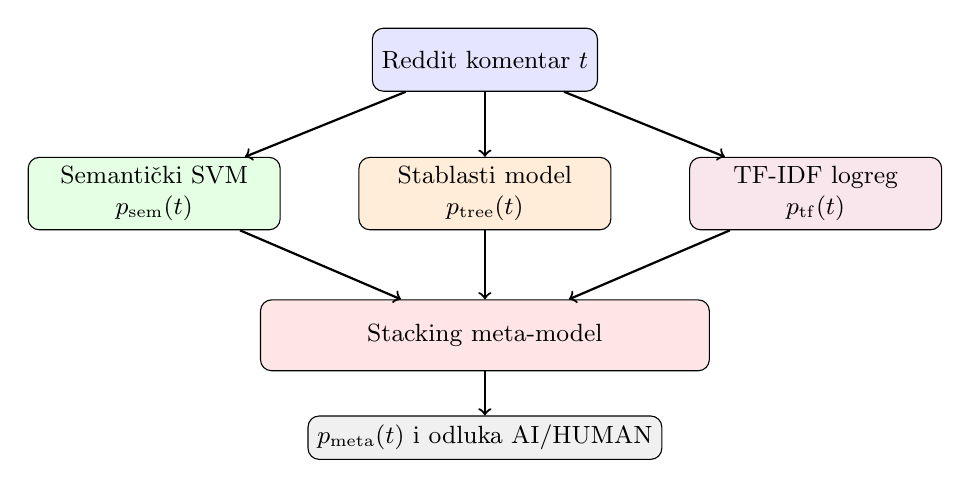
\begin{tikzpicture}[every node/.style={font=\small, align=center}]
        \node[draw, rounded corners, fill=blue!10, minimum width=2.8cm, minimum height=8mm] (text) at (0,0) {Reddit komentar $t$};
        \node[draw, rounded corners, fill=green!10, minimum width=3.2cm] (sem) at (-4.2,-1.7) {Semantički SVM\\$p_{\mathrm{sem}}(t)$};
        \node[draw, rounded corners, fill=orange!15, minimum width=3.2cm] (tree) at (0,-1.7) {Stablasti model\\$p_{\mathrm{tree}}(t)$};
        \node[draw, rounded corners, fill=purple!10, minimum width=3.2cm] (tf) at (4.2,-1.7) {TF-IDF logreg\\$p_{\mathrm{tf}}(t)$};
        \node[draw, rounded corners, fill=red!10, minimum width=5.7cm, minimum height=9mm] (meta) at (0,-3.5) {Stacking meta-model};
        \node[draw, rounded corners, fill=gray!12, minimum width=4.2cm] (out) at (0,-4.8) {$p_{\mathrm{meta}}(t)$ i odluka AI/HUMAN};
        \draw[->, thick] (text) -- (sem);
        \draw[->, thick] (text) -- (tree);
        \draw[->, thick] (text) -- (tf);
        \draw[->, thick] (sem) -- (meta);
        \draw[->, thick] (tree) -- (meta);
        \draw[->, thick] (tf) -- (meta);
        \draw[->, thick] (meta) -- (out);
    \end{tikzpicture}

    \vspace{2mm}
    {\small Tri komplementarna pogleda: značenje, struktura i lokalni tekstualni obrasci.}
\end{frame}

\begin{frame}{Formalizacija zadatka}
    \begin{columns}[T]
        \begin{column}{0.50\textwidth}
            \[
                y=1 \Leftrightarrow \texttt{AI}, \qquad y=0 \Leftrightarrow \texttt{HUMAN}
            \]

            \[
                p(t) \approx P(y=1\mid t)
            \]

            \[
                \hat y=\mathbf{1}\{p(t)\ge 0.5\}
            \]
        \end{column}
        \begin{column}{0.46\textwidth}
            \begin{tabular}{@{}ll@{}}
                \toprule
                \textbf{Podsustav} & \textbf{Signal} \\ \midrule
                SVM & semantički embedding \\
                Stabla & 20 strukturnih značajki \\
                TF-IDF & 1.56M rijetkih $n$-grama \\
                Meta-model & kombinacija vjerojatnosti \\ \bottomrule
            \end{tabular}
        \end{column}
    \end{columns}
\end{frame}

\section{Semantički SVM}

\begin{frame}{Model 1: Semantički SVM}
    \begin{columns}[T]
        \begin{column}{0.49\textwidth}
            \textbf{Prikaz komentara}
            \[
                \hat{x}=\frac{x}{\|x\|_2}, \qquad
                z_j=\frac{\hat{x}_j-\mu_j}{\sigma_j}
            \]

            \textbf{Linearna odluka}
            \[
                f(z)=w^\top z+b
            \]

            \[
                p_{\mathrm{sem}}(t)\approx P(y=1\mid t)
            \]
        \end{column}
        \begin{column}{0.47\textwidth}
            \small
            \begin{itemize}
                \item Embedding model mapira tekst u prostor značenja.
                \item \texttt{LinearSVC} razdvaja standardizirane embeddinge.
                \item Vjerojatnost se dobiva Plattovom kalibracijom.
            \end{itemize}

            \[
                P(y=1\mid s)\approx \frac{1}{1+\exp(As+B)}
            \]
        \end{column}
    \end{columns}
\end{frame}

\begin{frame}{Semantički SVM: margina i rezultati}
    \begin{columns}[T]
        \begin{column}{0.45\textwidth}
            \[
                \min_{w,b}\;\frac{1}{2}\|w\|_2^2 + C\sum_{i=1}^{n}\max\{0,1-\tilde y_i(w^\top z_i+b)\}
            \]

            \[
                \text{širina margine}=\frac{2}{\|w\|_2}
            \]
        \end{column}
        \begin{column}{0.51\textwidth}
            \centering
            \small
            \begin{tabular}{@{}lc@{}}
                \toprule
                \textbf{Metrika} & \textbf{Dev} \\ \midrule
                Točnost & 0.90948 \\
                Preciznost & 0.90341 \\
                Odziv & 0.91283 \\
                $F_1$ & 0.90810 \\
                ROC AUC & 0.96885 \\ \bottomrule
            \end{tabular}

            \vspace{2mm}
            \begin{tabular}{@{}lcc@{}}
                \toprule
                & $\hat y=0$ & $\hat y=1$ \\ \midrule
                $y=0$ & 19549 & 2022 \\
                $y=1$ & 1806 & 18912 \\ \bottomrule
            \end{tabular}
        \end{column}
    \end{columns}
\end{frame}

\section{Stablasti Model}

\begin{frame}{Model 2: Stablasti model}
    \begin{columns}[T]
        \begin{column}{0.48\textwidth}
            \textbf{Ulaz}
            \[
                x\in\mathbb{R}^{20}
            \]

            \small
            Značajke: broj riječi i rečenica po odlomku, upitnici, apostrofi, zagrade, crtice, duljine rečenica, prijelazne riječi i brojčane reference.
        \end{column}
        \begin{column}{0.48\textwidth}
            \textbf{Ansambl stabala}
            \[
                F_M(x)=\beta_0+\eta\sum_{m=1}^{M}T_m(x)
            \]

            \[
                p_{\mathrm{tree}}(x)=\frac{1}{1+e^{-F_M(x)}}
            \]

            \small \texttt{HistGradientBoostingClassifier}: dubina 5, stopa učenja 0.06, 300 iteracija.
        \end{column}
    \end{columns}
\end{frame}

\begin{frame}{Stablasti model: najvažnije značajke}
    \centering
    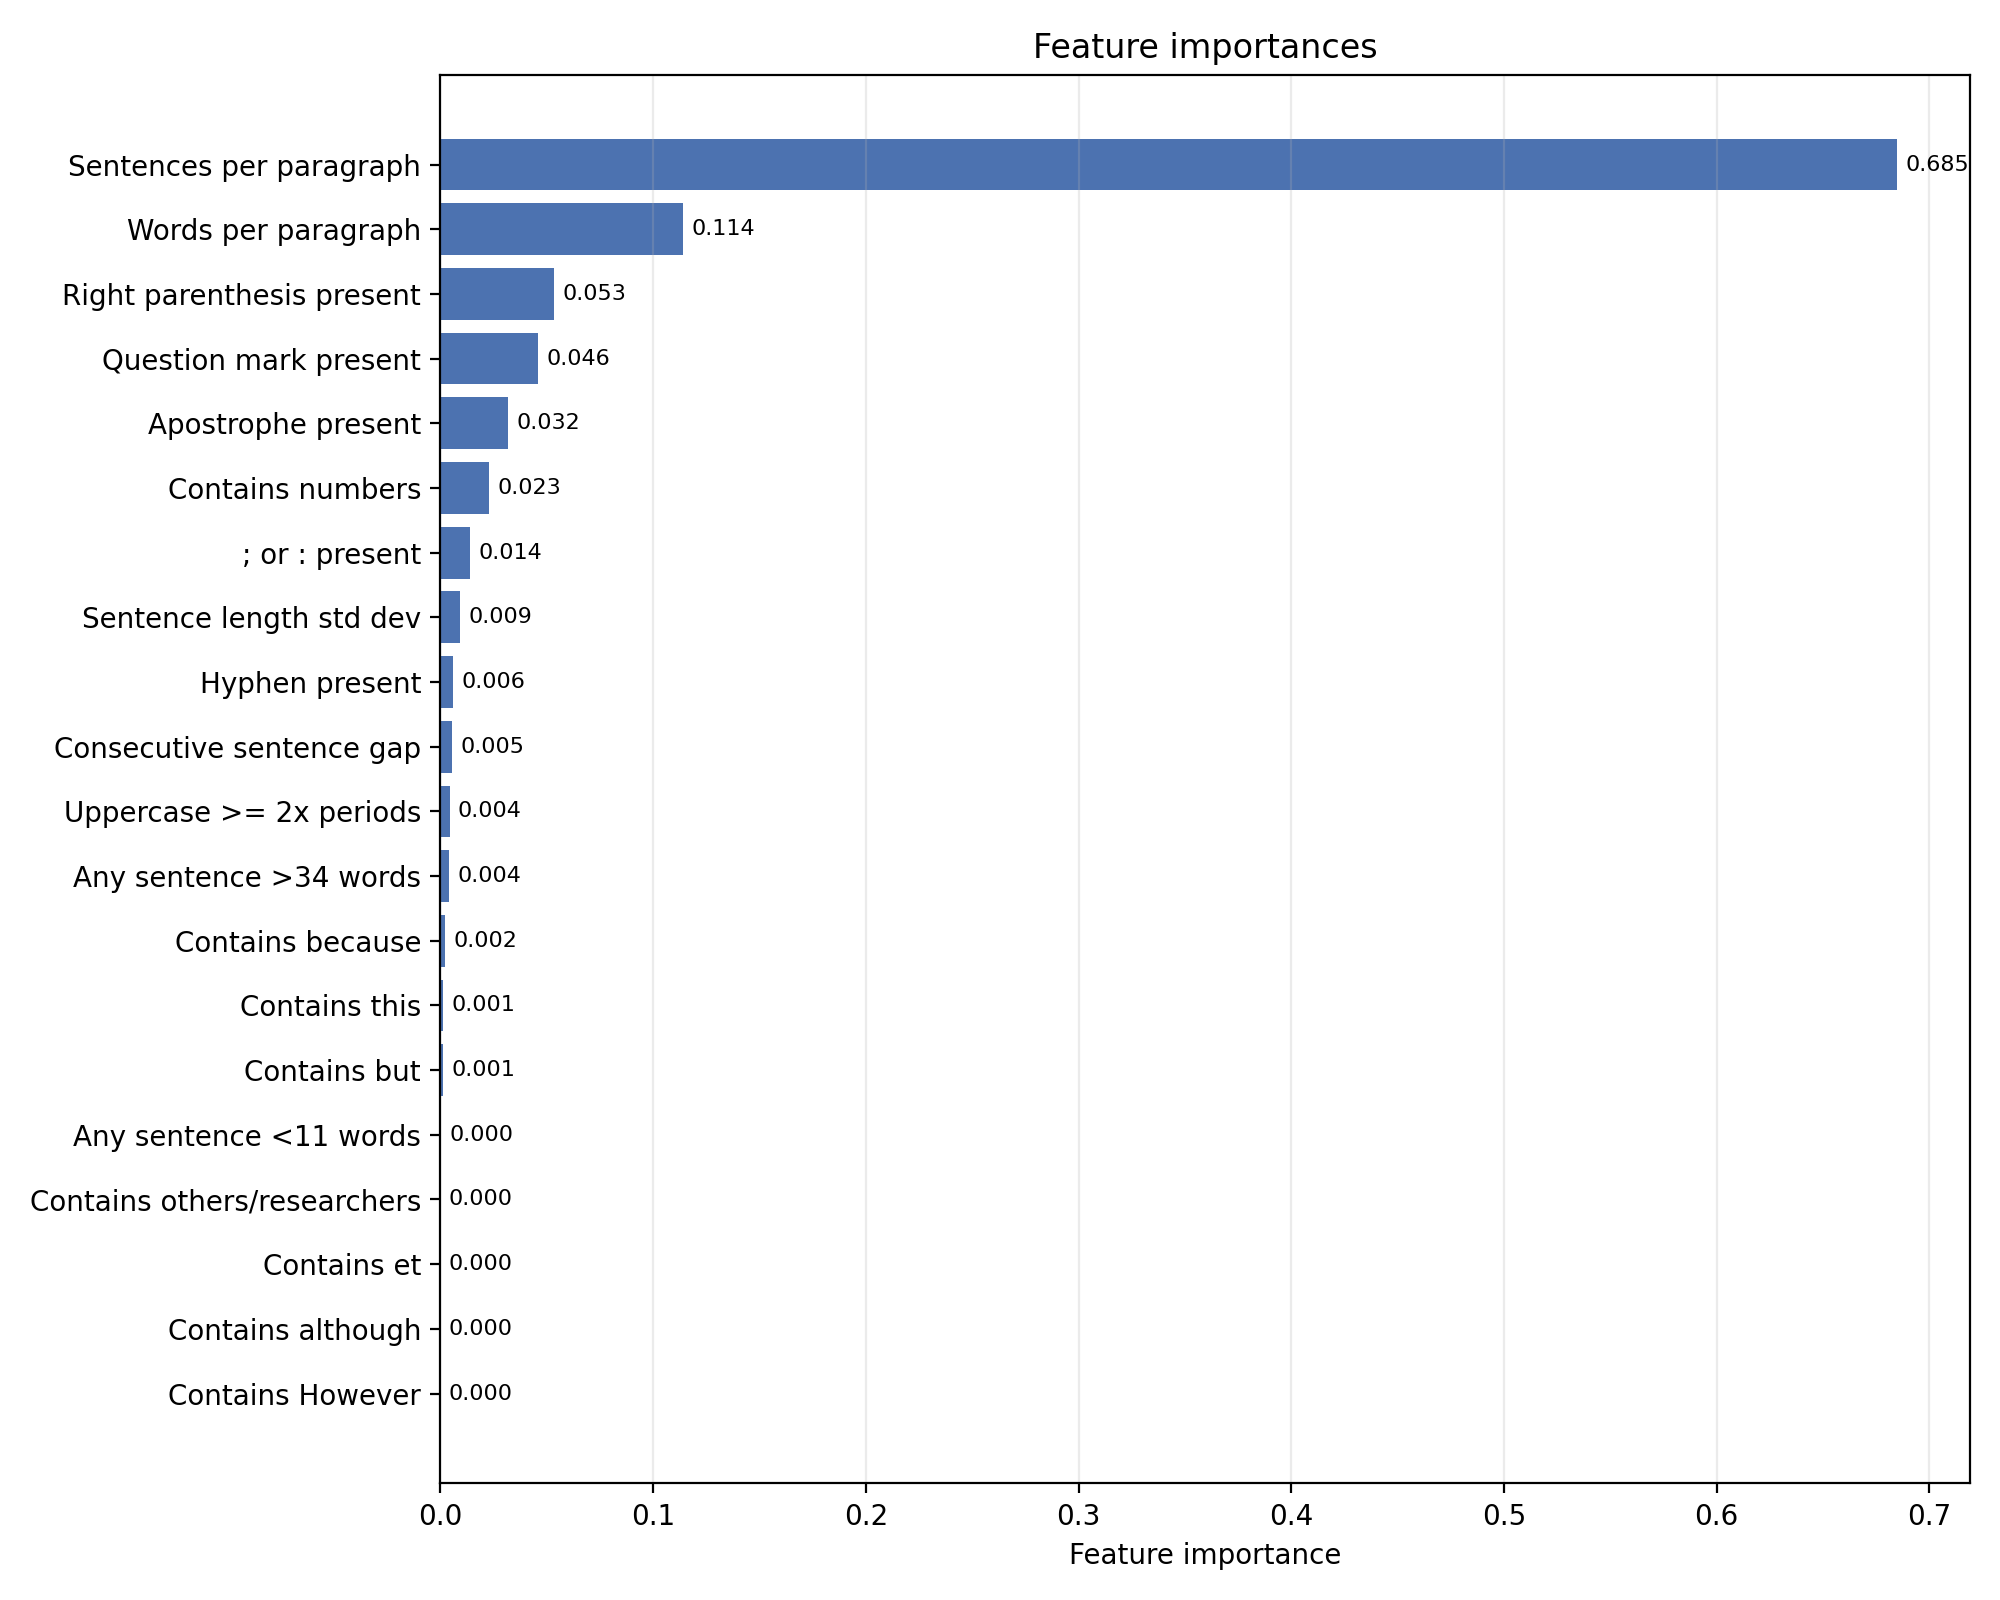
\includegraphics[width=0.82\textwidth,height=0.67\textheight,keepaspectratio]{../Tree_Based_Model/artifacts/tree_based_feature_importances.png}

    \vspace{1mm}
    {\small Najveći doprinos: broj riječi po odlomku, broj rečenica po odlomku, apostrofi, upitnici i varijabilnost duljine rečenica.}
\end{frame}

\begin{frame}{Stablasti model: rezultati}
    \centering
    \begin{columns}[T]
        \begin{column}{0.48\textwidth}
            \begin{tabular}{@{}lc@{}}
                \toprule
                \textbf{Metrika} & \textbf{Dev} \\ \midrule
                Točnost & 0.90487 \\
                Uravnotežena točnost & 0.9051 \\
                Preciznost & 0.89214 \\
                Odziv & 0.91664 \\
                $F_1$ & 0.90423 \\
                ROC AUC & 0.96696 \\ \bottomrule
            \end{tabular}
        \end{column}
        \begin{column}{0.45\textwidth}
            \begin{tabular}{@{}lcc@{}}
                \toprule
                & $\hat y=0$ & $\hat y=1$ \\ \midrule
                $y=0$ & 19275 & 2296 \\
                $y=1$ & 1727 & 18991 \\ \bottomrule
            \end{tabular}
        \end{column}
    \end{columns}
\end{frame}

\section{TF-IDF Logistička Regresija}

\begin{frame}{Model 3: TF-IDF logistička regresija}
    \begin{columns}[T]
        \begin{column}{0.48\textwidth}
            \textbf{TF-IDF}
            \[
                \operatorname{tf}(t,g)=1+\log c_{t,g}
            \]

            \[
                \operatorname{idf}(g)=\log\frac{1+N}{1+\operatorname{df}(g)}+1
            \]

            \[
                \tilde x_g(t)=\operatorname{tf}(t,g)\operatorname{idf}(g)
            \]
        \end{column}
        \begin{column}{0.48\textwidth}
            \textbf{Dvije vrste $n$-grama}
            \begin{tabular}{@{}ll@{}}
                \toprule
                Riječi & 1--2 grama \\
                Znakovi & 3--5 grama \\
                \bottomrule
            \end{tabular}

            \vspace{3mm}
            \[
                x(t)=\begin{bmatrix}x_{\mathrm{word}}(t)\\x_{\mathrm{char}}(t)\end{bmatrix}\in\mathbb{R}^{1557681}
            \]
        \end{column}
    \end{columns}
\end{frame}

\begin{frame}{TF-IDF logistička regresija: odluka i gubitak}
    \begin{columns}[T]
        \begin{column}{0.48\textwidth}
            \[
                s_c(x)=w_c^\top x+b_c
            \]

            \[
                p_{\mathrm{tf}}(t)=\frac{\exp(s_{\texttt{AI}}(x(t)))}{\exp(s_{\texttt{AI}}(x(t)))+\exp(s_{\texttt{HUMAN}}(x(t)))}
            \]
        \end{column}
        \begin{column}{0.48\textwidth}
            \[
                \min_w\sum_{i=1}^{n}\alpha_{y_i}\left[-y_i\log p_i-(1-y_i)\log(1-p_i)\right]+\lambda\|w\|_2^2
            \]

            \small Koristi se \texttt{class\_weight=balanced}; rjeđi razred dobiva veću težinu u gubitku.
        \end{column}
    \end{columns}
\end{frame}

\begin{frame}{TF-IDF logistička regresija: rezultati}
    \centering
    \begin{columns}[T]
        \begin{column}{0.48\textwidth}
            \begin{tabular}{@{}lc@{}}
                \toprule
                \textbf{Metrika} & \textbf{Dev} \\ \midrule
                Točnost & 0.98085 \\
                Preciznost & 0.98627 \\
                Odziv & 0.97447 \\
                $F_1$ & 0.98033 \\
                ROC AUC & 0.99780 \\
                Log-gubitak & 0.06739 \\
                Brier & 0.01626 \\ \bottomrule
            \end{tabular}
        \end{column}
        \begin{column}{0.45\textwidth}
            \begin{tabular}{@{}lcc@{}}
                \toprule
                & $\hat y=0$ & $\hat y=1$ \\ \midrule
                $y=0$ & 21290 & 281 \\
                $y=1$ & 529 & 20189 \\ \bottomrule
            \end{tabular}

            \vspace{3mm}
            \small Najjači pojedinačni bazni model.
        \end{column}
    \end{columns}
\end{frame}

\section{Stacking Meta-Model}

\begin{frame}{Stacking: kako spajamo tri modela}
    \begin{columns}[T]
        \begin{column}{0.48\textwidth}
            \[
                p_{\mathrm{sem}}(t),\qquad p_{\mathrm{tree}}(t),\qquad p_{\mathrm{tf}}(t)
            \]

            \[
                p_{\mathrm{meta}}(t)\approx P(y=1\mid p_{\mathrm{sem}},p_{\mathrm{tree}},p_{\mathrm{tf}})
            \]
        \end{column}
        \begin{column}{0.48\textwidth}
            \small
            \begin{itemize}
                \item Train ulazi za meta-model dobiveni su out-of-fold postupkom.
                \item Finalni bazni modeli treniraju se na cijelom train skupu.
                \item Meta-model je logistička regresija nad logitima i interakcijama.
            \end{itemize}
        \end{column}
    \end{columns}
\end{frame}

\begin{frame}{Meta-značajke}
    \[
        \ell_i=\log\frac{p_i}{1-p_i}, \qquad p_i\in[10^{-5},1-10^{-5}]
    \]

    \[
        \ell_1=\operatorname{logit}(p_{\mathrm{sem}}),\quad
        \ell_2=\operatorname{logit}(p_{\mathrm{tree}}),\quad
        \ell_3=\operatorname{logit}(p_{\mathrm{tf}})
    \]

    \[
        \phi(t)=\left[\ell_1,\ell_2,\ell_3,\ell_1\ell_2,\ell_1\ell_3,\ell_2\ell_3,\ell_1^2,\ell_2^2,\ell_3^2\right]
    \]
\end{frame}

\begin{frame}{Završna funkcija odluke}
    \[
        p_{\mathrm{meta}}(t)=\sigma\left(\beta_0+\sum_{i=1}^{3}\beta_i\ell_i+\sum_{i<j}\beta_{ij}\ell_i\ell_j+\sum_{i=1}^{3}\gamma_i\ell_i^2\right)
    \]

    \[
        \sigma(u)=\frac{1}{1+e^{-u}}, \qquad
        \hat y=\mathbf{1}\{p_{\mathrm{meta}}(t)\ge 0.5\}
    \]

    \vspace{2mm}
    \centering
    {\small Interakcije dopuštaju modelu da razlikuje slaganje i proturječje baznih podsustava.}
\end{frame}

\section{Rezultati}

\begin{frame}{Usporedba modela na razvojnom skupu}
    \centering
    \scriptsize
    \setlength{\tabcolsep}{3.4pt}
    \begin{tabular}{@{}lccccccc@{}}
        \toprule
        \textbf{Model} & \textbf{Točnost} & \textbf{Prec.} & \textbf{Odziv} & \textbf{$F_1$} & \textbf{AUC} & \textbf{Log-gub.} & \textbf{Brier} \\ \midrule
        Semantički SVM & 0.90948 & 0.90341 & 0.91283 & 0.90810 & 0.96885 & 0.22646 & 0.06715 \\
        Stablasti model & 0.90487 & 0.89214 & 0.91664 & 0.90423 & 0.96696 & 0.23115 & 0.07009 \\
        TF-IDF logreg & 0.98085 & 0.98627 & 0.97447 & 0.98033 & 0.99780 & 0.06739 & 0.01626 \\
        \midrule
        \textbf{Meta-model} & \textbf{0.98406} & \textbf{0.98788} & \textbf{0.97949} & \textbf{0.98366} & \textbf{0.99840} & \textbf{0.04564} & \textbf{0.01240} \\ \bottomrule
    \end{tabular}

    \vspace{3mm}
    \small Meta-model je najbolji po svim navedenim metrikama.
\end{frame}

\begin{frame}{Konfuzijske matrice na razvojnom skupu}
    \centering
    \scriptsize
    \begin{tabular}{@{}lrrrr@{}}
        \toprule
        \textbf{Model} & \textbf{TN} & \textbf{FP} & \textbf{FN} & \textbf{TP} \\ \midrule
        Semantički SVM & 19549 & 2022 & 1806 & 18912 \\
        Stablasti model & 19275 & 2296 & 1727 & 18991 \\
        TF-IDF logreg & 21290 & 281 & 529 & 20189 \\
        \textbf{Meta-model} & \textbf{21322} & \textbf{249} & \textbf{425} & \textbf{20293} \\ \bottomrule
    \end{tabular}

    \vspace{5mm}
    \begin{columns}[T]
        \begin{column}{0.47\textwidth}
            \centering
            \textbf{Meta-model}
            \[
            \begin{array}{c|cc}
             & \hat y=0 & \hat y=1 \\
            \hline
            y=0 & 21322 & 249 \\
            y=1 & 425 & 20293
            \end{array}
            \]
        \end{column}
        \begin{column}{0.47\textwidth}
            \small
            Meta-model smanjuje i lažno pozitivne i lažno negativne primjere u odnosu na najjači pojedinačni model.
        \end{column}
    \end{columns}
\end{frame}

\begin{frame}{Test rezultat završnog modela}
    \centering
    \begin{tabular}{@{}ccccccc@{}}
        \toprule
        \textbf{Točnost} & \textbf{Prec.} & \textbf{Odziv} & \textbf{$F_1$} & \textbf{AUC} & \textbf{Log-gub.} & \textbf{Brier} \\ \midrule
        0.98406 & 0.98722 & 0.98016 & 0.98368 & 0.99842 & 0.04499 & 0.01226 \\ \bottomrule
    \end{tabular}

    \vspace{7mm}
    \Large
    \[
        p_{\mathrm{meta}}(t) \in [0,1]
    \]

    \normalsize
    Završni izlaz nije samo oznaka, nego procjena vjerojatnosti AI autorstva.
\end{frame}

\begin{frame}{Zaključak}
    \begin{itemize}
        \item Koristimo točno tri bazna modela: semantički SVM, stablasti model i TF-IDF logističku regresiju.
        \item Modeli gledaju različite signale: značenje, strukturu i lokalne tekstualne obrasce.
        \item Stacking meta-model kombinira njihove vjerojatnosti preko logita, interakcija i kvadratnih članova.
        \item Završni model postiže najbolji rezultat: dev accuracy $0.98406$, test accuracy $0.98406$.
        \item Sustav procjenjuje vjerojatnost AI-generiranosti komentara, a ne dokazuje identitet autora.
    \end{itemize}
\end{frame}

\end{document}
